\documentclass[11pt, a4paper]{article}

% Fonts and Encoding
\usepackage[utf8]{inputenc}
\usepackage[T1]{fontenc}

% Math and Symbols
\usepackage{amsmath, amssymb, amsthm, amsfonts, mathrsfs, mathtools}

% Layout and Geometry
\usepackage{geometry}
\geometry{a4paper, margin=1in}

% Formatting and Graphics
\usepackage{graphicx, xcolor, enumitem, booktabs, array, tabularx}

% TikZ for Illustrations
\usepackage{tikz}
\usetikzlibrary{arrows.meta, positioning, shapes.geometric, calc, backgrounds, matrix}

% Clickable Links and TOC
\usepackage{hyperref}
\hypersetup{
    colorlinks=true,
    linkcolor=blue,
    filecolor=magenta,      
    urlcolor=cyan,
    pdftitle={Advanced Mathematics Topic},
}

% Theorem Environments
\newtheorem{theorem}{Theorem}[section]
\newtheorem{lemma}[theorem]{Lemma}
\newtheorem{proposition}[theorem]{Proposition}
\newtheorem{corollary}[theorem]{Corollary}
\theoremstyle{definition}
\newtheorem{definition}{Definition}[section]
\newtheorem{axiom}{Axiom}[section]
\newtheorem{example}{Example}[section]
\theoremstyle{remark}
\newtheorem{remark}{Remark}[section]

% Custom Commands (Enforced standard notation)
\newcommand{\R}{\mathbb{R}}
\newcommand{\N}{\mathbb{N}}
\newcommand{\Z}{\mathbb{Z}}
\newcommand{\Q}{\mathbb{Q}}
\newcommand{\E}{\mathbb{E}}
\newcommand{\Prob}{\mathbb{P}}
\newcommand{\F}{\mathcal{F}}

\begin{document}

\title{\textbf{Mastering The Strong Principle of Mathematical Induction}\\
\large Bridging Abstract Logic to Advanced Quantitative Modeling}
\author{Tashfeen Omran}
\date{\today}

\maketitle

\tableofcontents
\newpage

% ==========================================
% PART 1: INTRODUCTION
% ==========================================
\section{Part 1: Comprehensive Introduction, Context, and Prerequisites}

\subsection{Core Concepts \& Axioms}
Mathematical Induction is a foundational proof technique used to establish the truth of an infinite sequence of propositions, typically indexed by the natural numbers $\N$. While the Standard (or Weak) Principle of Mathematical Induction relies on the truth of a proposition $P(k)$ to prove $P(k+1)$, the \textbf{Strong Principle of Mathematical Induction} (also known as Complete Induction) leverages a more robust hypothesis. It asserts that to prove $P(k+1)$, one may assume the truth of $P(i)$ for \textit{all} integers $i$ such that $m \le i \le k$, where $m$ is the base case.

Formally, let $P(n)$ be a statement defined for integers $n \ge m$. The Strong Principle of Mathematical Induction states that if:
\begin{enumerate}
    \item \textbf{Base Case(s):} $P(m), P(m+1), \dots, P(m+j)$ are true for some $j \ge 0$.
    \item \textbf{Inductive Step:} For any integer $k \ge m+j$, the assumption that $P(i)$ is true for all $i \in \{m, m+1, \dots, k\}$ implies that $P(k+1)$ is true.
\end{enumerate}
Then, $P(n)$ is true for all integers $n \ge m$.

\subsection{Intuition and Set-Theoretic Foundations}
Intuitively, standard induction is like a line of falling dominoes where each domino only needs the immediately preceding domino to knock it over. Strong induction, however, is akin to a domino that requires the combined weight or momentum of \textit{all} preceding dominoes to fall. 

From a set-theoretic perspective, both forms of induction are logically equivalent to the \textbf{Well-Ordering Principle} of the natural numbers, which states that every non-empty subset of $\N$ has a least element. If a proposition $P(n)$ were false for some $n$, the set of counterexamples $S = \{n \in \N : \neg P(n)\}$ would be non-empty and thus have a least element, say $x$. Strong induction essentially proves that $x$ cannot exist, because the truth of $P$ for all elements strictly less than $x$ forces $P(x)$ to be true, creating a contradiction.

\subsection{Historical Context and Motivation}
The formalization of induction dates back to the works of Blaise Pascal and Pierre de Fermat in the 17th century, primarily motivated by early probability theory and combinatorial games. However, the necessity for \textit{Strong} Induction arose when mathematicians began formalizing Number Theory (e.g., the Fundamental Theorem of Arithmetic). Proving that every integer can be factored into primes requires Strong Induction because an integer $n$ factors into two smaller integers $a$ and $b$, which are not necessarily $n-1$. Thus, knowing the theorem holds for $n-1$ is useless; one must know it holds for all integers smaller than $n$.

\subsection{Key Theorems and Logical Equivalences}
\begin{theorem}[Equivalence of Induction Principles]
    The following three statements are logically equivalent within the standard axioms of arithmetic (Peano Axioms):
    \begin{itemize}
        \item The Well-Ordering Principle.
        \item The Principle of Mathematical Induction (Weak).
        \item The Strong Principle of Mathematical Induction.
    \end{itemize}
\end{theorem}

\subsection{Prerequisites}
To master this chapter, the reader must possess:
\begin{itemize}
    \item \textbf{Foundational Logic:} Understanding of implications ($A \implies B$), logical AND ($\land$), and quantifiers ($\forall, \exists$).
    \item \textbf{Algebraic Manipulation:} Proficiency in factoring polynomials, handling inequalities, and manipulating indices in summations.
    \item \textbf{Modular Arithmetic:} Basic understanding of divisibility (denoted $a \mid b$) and congruences.
\end{itemize}

% ==========================================
% PART 2: HOMEWORK SOLUTIONS
% ==========================================
\section{Part 2: Detailed Homework Solutions}

This section provides rigorous, step-by-step proofs for Exercises 6.33 through 6.39 from the provided text.

\subsection{Exercise 6.33}
\textbf{Problem:} A sequence $\{a_n\}$ is defined recursively by $a_1 = 1$ and $a_n = 2a_{n-1}$ for $n \ge 2$. Conjecture a formula for $a_n$ and verify that your conjecture is correct.

\textbf{Conjecture:} 
Computing the first few terms: $a_1 = 1$, $a_2 = 2(1) = 2$, $a_3 = 2(2) = 4$, $a_4 = 2(4) = 8$. 
We conjecture that $a_n = 2^{n-1}$ for all integers $n \ge 1$.

\begin{proof}
    We proceed by Mathematical Induction on $n$. Let $P(n)$ be the statement that $a_n = 2^{n-1}$.
    
    \textbf{Base Case ($n=1$):} 
    By definition, $a_1 = 1$. Using our formula, $2^{1-1} = 2^0 = 1$. Thus, $P(1)$ is true.
    
    \textbf{Inductive Step:} 
    Assume that $P(k)$ is true for an arbitrary integer $k \ge 1$. That is, assume $a_k = 2^{k-1}$. We must show that $P(k+1)$ is true, meaning $a_{k+1} = 2^k$.
    
    By the recursive definition of the sequence for $n \ge 2$, we have:
    \[ a_{k+1} = 2a_k \]
    Substituting the inductive hypothesis $a_k = 2^{k-1}$ into the equation yields:
    \[ a_{k+1} = 2 \cdot (2^{k-1}) = 2^1 \cdot 2^{k-1} = 2^k \]
    This establishes $P(k+1)$. By the Principle of Mathematical Induction, $a_n = 2^{n-1}$ for all integers $n \ge 1$.
\end{proof}

\subsection{Exercise 6.34}
\textbf{Problem:} A sequence $\{a_n\}$ is defined recursively by $a_1 = 1, a_2 = 2$ and $a_n = a_{n-1} + 2a_{n-2}$ for $n \ge 3$. Conjecture a formula for $a_n$ and verify that your conjecture is correct.

\textbf{Conjecture:}
Computing the first few terms:
$a_1 = 1$ \\
$a_2 = 2$ \\
$a_3 = a_2 + 2a_1 = 2 + 2(1) = 4$ \\
$a_4 = a_3 + 2a_2 = 4 + 2(2) = 8$ \\
$a_5 = a_4 + 2a_3 = 8 + 2(4) = 16$ \\
We conjecture that $a_n = 2^{n-1}$ for all integers $n \ge 1$.

\begin{proof}
    We proceed by the Strong Principle of Mathematical Induction. Let $P(n)$ be the statement that $a_n = 2^{n-1}$.
    
    \textbf{Base Cases ($n=1, 2$):}
    For $n=1$, $a_1 = 1$ and $2^{1-1} = 1$. $P(1)$ is true.
    For $n=2$, $a_2 = 2$ and $2^{2-1} = 2$. $P(2)$ is true.
    
    \textbf{Inductive Step:}
    Assume that $P(i)$ is true for all integers $i$ such that $1 \le i \le k$, where $k \ge 2$. We must show that $P(k+1)$ is true, meaning $a_{k+1} = 2^k$.
    
    Since $k \ge 2$, $k+1 \ge 3$. By the recursive definition:
    \[ a_{k+1} = a_k + 2a_{k-1} \]
    By our strong inductive hypothesis, we know $a_k = 2^{k-1}$ and $a_{k-1} = 2^{k-2}$. Substituting these into the equation:
    \begin{align*}
        a_{k+1} &= 2^{k-1} + 2(2^{k-2}) \\
        &= 2^{k-1} + 2^{k-1} \\
        &= 2 \cdot 2^{k-1} \\
        &= 2^k
    \end{align*}
    This establishes $P(k+1)$. By the Strong Principle of Mathematical Induction, $a_n = 2^{n-1}$ for all integers $n \ge 1$.
\end{proof}

\subsection{Exercise 6.35}
\textbf{Problem:} A sequence $\{a_n\}$ is defined recursively by $a_1 = 1, a_2 = 4, a_3 = 9$ and $a_n = a_{n-1} - a_{n-2} + a_{n-3} + 2(2n-3)$ for $n \ge 4$. Conjecture a formula for $a_n$ and prove that your conjecture is correct.

\textbf{Conjecture:}
The first three terms are $1^2, 2^2, 3^2$. Let us compute $a_4$ to verify:
\[ a_4 = a_3 - a_2 + a_1 + 2(2(4)-3) = 9 - 4 + 1 + 2(5) = 6 + 10 = 16 = 4^2 \]
We conjecture that $a_n = n^2$ for all integers $n \ge 1$.

\begin{proof}
    We proceed by the Strong Principle of Mathematical Induction. Let $P(n)$ be the statement that $a_n = n^2$.
    
    \textbf{Base Cases ($n=1, 2, 3$):}
    $a_1 = 1 = 1^2$, $a_2 = 4 = 2^2$, $a_3 = 9 = 3^2$. Thus, $P(1), P(2),$ and $P(3)$ are true.
    
    \textbf{Inductive Step:}
    Assume that $P(i)$ is true for all integers $i$ such that $1 \le i \le k$, where $k \ge 3$. We must show that $P(k+1)$ is true, meaning $a_{k+1} = (k+1)^2$.
    
    Since $k \ge 3$, $k+1 \ge 4$. By the recursive definition:
    \[ a_{k+1} = a_k - a_{k-1} + a_{k-2} + 2(2(k+1)-3) \]
    By the strong inductive hypothesis, $a_k = k^2$, $a_{k-1} = (k-1)^2$, and $a_{k-2} = (k-2)^2$. Substituting these yields:
    \begin{align*}
        a_{k+1} &= k^2 - (k-1)^2 + (k-2)^2 + 2(2k - 1) \\
        &= k^2 - (k^2 - 2k + 1) + (k^2 - 4k + 4) + 4k - 2 \\
        &= k^2 - k^2 + 2k - 1 + k^2 - 4k + 4 + 4k - 2 \\
        &= k^2 + (2k - 4k + 4k) + (-1 + 4 - 2) \\
        &= k^2 + 2k + 1 \\
        &= (k+1)^2
    \end{align*}
    This establishes $P(k+1)$. By the Strong Principle of Mathematical Induction, $a_n = n^2$ for all integers $n \ge 1$.
\end{proof}

\subsection{Exercise 6.36}
\textbf{Problem:} Consider the sequence $F_1, F_2, F_3, \dots$ where $F_1 = 1, F_2 = 1, F_3 = 2, F_4 = 3, F_5 = 5, F_6 = 8$.
(a) Define the sequence of Fibonacci numbers by means of a recurrence relation.
(b) Prove that $2 \mid F_n$ if and only if $3 \mid n$.

\textbf{Solution (a):}
The Fibonacci sequence is defined recursively by:
$F_1 = 1$, $F_2 = 1$, and $F_n = F_{n-1} + F_{n-2}$ for all integers $n \ge 3$.

\textbf{Solution (b):}
\begin{proof}
    We proceed by the Strong Principle of Mathematical Induction on $n$. Let $P(n)$ be the biconditional statement: $2 \mid F_n \iff 3 \mid n$.
    
    \textbf{Base Cases ($n=1, 2, 3$):}
    For $n=1$: $F_1 = 1$. $2 \nmid 1$ and $3 \nmid 1$. Both sides are false, so the biconditional is true.
    For $n=2$: $F_2 = 1$. $2 \nmid 1$ and $3 \nmid 2$. Both sides are false, so the biconditional is true.
    For $n=3$: $F_3 = 2$. $2 \mid 2$ and $3 \mid 3$. Both sides are true, so the biconditional is true.
    
    \textbf{Inductive Step:}
    Assume that $P(i)$ is true for all integers $i$ such that $1 \le i \le k$, where $k \ge 3$. We must show that $P(k+1)$ is true, meaning $2 \mid F_{k+1} \iff 3 \mid (k+1)$.
    
    By the recurrence relation, we can express $F_{k+1}$ in terms of earlier elements:
    \begin{align*}
        F_{k+1} &= F_k + F_{k-1} \\
        &= (F_{k-1} + F_{k-2}) + F_{k-1} \quad \text{(since $k \ge 3$)} \\
        &= 2F_{k-1} + F_{k-2}
    \end{align*}
    Since $2F_{k-1}$ is an even integer, the parity of $F_{k+1}$ is entirely determined by the parity of $F_{k-2}$. Therefore:
    \[ 2 \mid F_{k+1} \iff 2 \mid F_{k-2} \]
    By our strong inductive hypothesis, $P(k-2)$ is true (since $1 \le k-2 \le k$). Thus:
    \[ 2 \mid F_{k-2} \iff 3 \mid (k-2) \]
    Furthermore, in modular arithmetic, $(k-2) \equiv (k+1) \pmod 3$. Therefore:
    \[ 3 \mid (k-2) \iff 3 \mid (k+1) \]
    Chaining these logical equivalences together yields:
    \[ 2 \mid F_{k+1} \iff 2 \mid F_{k-2} \iff 3 \mid (k-2) \iff 3 \mid (k+1) \]
    This establishes $P(k+1)$. By the Strong Principle of Mathematical Induction, $2 \mid F_n \iff 3 \mid n$ for all integers $n \ge 1$.
\end{proof}

\subsection{Exercise 6.37}
\textbf{Problem:} Prove the following statement: For each integer $n \ge 12$, there exist nonnegative integers $a$ and $b$ such that $n = 3a + 7b$. Use the Strong Principle of Mathematical Induction.

\begin{proof}
    Let $P(n)$ be the statement that there exist nonnegative integers $a$ and $b$ such that $n = 3a + 7b$. We proceed by Strong Induction for $n \ge 12$.
    
    \textbf{Base Cases ($n=12, 13, 14$):}
    For $n=12$: $12 = 3(4) + 7(0)$. Here $a=4, b=0 \ge 0$. $P(12)$ is true.
    For $n=13$: $13 = 3(2) + 7(1)$. Here $a=2, b=1 \ge 0$. $P(13)$ is true.
    For $n=14$: $14 = 3(0) + 7(2)$. Here $a=0, b=2 \ge 0$. $P(14)$ is true.
    
    \textbf{Inductive Step:}
    Assume that $P(i)$ is true for all integers $i$ such that $12 \le i \le k$, where $k \ge 14$. We must show that $P(k+1)$ is true.
    
    Consider the integer $k+1$. Since $k \ge 14$, it follows that $(k+1) - 3 = k - 2 \ge 12$. 
    Because $12 \le k-2 \le k$, we can apply the strong inductive hypothesis to $k-2$. Thus, there exist nonnegative integers $x$ and $y$ such that:
    \[ k - 2 = 3x + 7y \]
    Adding 3 to both sides gives:
    \[ k + 1 = 3x + 7y + 3 = 3(x+1) + 7y \]
    Let $a = x+1$ and $b = y$. Since $x \ge 0$ and $y \ge 0$, it follows that $a \ge 1 > 0$ and $b \ge 0$. Thus, $k+1 = 3a + 7b$ for nonnegative integers $a, b$.
    This establishes $P(k+1)$. By the Strong Principle of Mathematical Induction, the statement holds for all integers $n \ge 12$.
\end{proof}

\subsection{Exercise 6.38}
\textbf{Problem:} Let $S = \{i \in \Z : i \ge 2\}$ and let $P$ be a subset of $S$ with the properties that $2, 3 \in P$ and if $n \in S$, then either $n \in P$ or $n = ab$, where $a, b \in S$. Prove that every element of $S$ either belongs to $P$ or can be expressed as a product of elements of $P$.

\begin{proof}
    We proceed by the Strong Principle of Mathematical Induction on $n \in S$. Let $Q(n)$ be the statement: "$n \in P$ or $n$ can be expressed as a product of elements of $P$."
    
    \textbf{Base Case ($n=2$):}
    We are given that $2 \in P$. Therefore, $Q(2)$ is trivially true.
    
    \textbf{Inductive Step:}
    Assume that $Q(i)$ is true for all integers $i$ such that $2 \le i \le k$, where $k \ge 2$. We must show that $Q(k+1)$ is true.
    
    Consider the integer $k+1 \in S$. By the given properties of $S$ and $P$, there are two mutually exclusive cases:
    \begin{itemize}
        \item \textbf{Case 1:} $k+1 \in P$. If this is true, then $Q(k+1)$ is immediately satisfied.
        \item \textbf{Case 2:} $k+1 \notin P$. By the given property, $k+1$ must be expressible as $k+1 = ab$, where $a, b \in S$. 
        Since $a, b \in S$, we know $a \ge 2$ and $b \ge 2$. 
        Because $a \ge 2$, it follows that $b = \frac{k+1}{a} \le \frac{k+1}{2} \le k$ (since $k \ge 2 \implies k+1 \le 2k$). 
        By symmetry, $a \le k$. 
        Thus, $2 \le a \le k$ and $2 \le b \le k$. 
        By our strong inductive hypothesis, $Q(a)$ and $Q(b)$ are both true. This means $a$ is either in $P$ or a product of elements of $P$, and the same is true for $b$. 
        Consequently, their product $ab = k+1$ is a product of elements of $P$.
    \end{itemize}
    In both cases, $Q(k+1)$ holds. By the Strong Principle of Mathematical Induction, $Q(n)$ is true for all $n \ge 2$.
\end{proof}

\subsection{Exercise 6.39}
\textbf{Problem:} Prove that there exists an odd integer $m$ such that every odd integer $n \ge m$ can be expressed as $3a + 11b$ or $5c + 7d$ for nonnegative integers $a, b, c$ and $d$.

\begin{proof}
    We will prove a stronger statement: There exists an odd integer $m = 21$ such that \textit{every} integer $n \ge 20$ can be expressed strictly in the form $3a + 11b$ for nonnegative integers $a, b$. If this holds, then trivially every odd integer $n \ge 21$ can be expressed as $3a + 11b$, satisfying the problem's condition.
    
    Let $P(n)$ be the statement that $n = 3a + 11b$ for nonnegative integers $a, b$. We proceed by Strong Induction for $n \ge 20$.
    
    \textbf{Base Cases ($n=20, 21, 22$):}
    For $n=20$: $20 = 3(3) + 11(1)$. Here $a=3, b=1 \ge 0$. $P(20)$ is true.
    For $n=21$: $21 = 3(7) + 11(0)$. Here $a=7, b=0 \ge 0$. $P(21)$ is true.
    For $n=22$: $22 = 3(0) + 11(2)$. Here $a=0, b=2 \ge 0$. $P(22)$ is true.
    
    \textbf{Inductive Step:}
    Assume that $P(i)$ is true for all integers $i$ such that $20 \le i \le k$, where $k \ge 22$. We must show that $P(k+1)$ is true.
    
    Consider the integer $k+1$. Since $k \ge 22$, it follows that $(k+1) - 3 = k - 2 \ge 20$.
    Because $20 \le k-2 \le k$, we can apply the strong inductive hypothesis to $k-2$. Thus, there exist nonnegative integers $x$ and $y$ such that:
    \[ k - 2 = 3x + 11y \]
    Adding 3 to both sides gives:
    \[ k + 1 = 3x + 11y + 3 = 3(x+1) + 11y \]
    Let $a = x+1$ and $b = y$. Since $x, y \ge 0$, we have $a \ge 1$ and $b \ge 0$. Thus, $k+1 = 3a + 11b$.
    
    This establishes $P(k+1)$. By Strong Induction, all integers $n \ge 20$ can be expressed as $3a + 11b$. Consequently, for the odd integer $m = 21$, every odd integer $n \ge m$ can be expressed as $3a + 11b$ (and we do not even need the $5c + 7d$ alternative).
\end{proof}

% ==========================================
% PART 3: IN-DEPTH ANALYSIS
% ==========================================
\section{Part 3: In-Depth Analysis of Problems and Techniques}

\subsection{A) Problem Types and Logical Strategies}
The exercises in this section fall into three distinct mathematical categories, each requiring a specific strategic approach:
\begin{enumerate}
    \item \textbf{Recursive Sequence Conjectures (6.33, 6.34, 6.35):} 
    \textit{Strategy:} Compute the first 4-5 terms to identify a pattern (e.g., powers of 2, perfect squares). The recurrence relation dictates the number of base cases required. If $a_n$ depends on $a_{n-1}, a_{n-2},$ and $a_{n-3}$, you \textit{must} establish three base cases ($n=1, 2, 3$) before the inductive step can safely look back three steps.
    \item \textbf{Divisibility and Modular Arithmetic (6.36):} 
    \textit{Strategy:} Instead of working with raw division, express the sequence algebraically to isolate the parity. In 6.36, proving $F_{k+1} = 2F_{k-1} + F_{k-2}$ was a critical strategic move because it immediately showed that $F_{k+1}$ and $F_{k-2}$ share the same parity, allowing a direct jump back to $P(k-2)$.
    \item \textbf{Frobenius Coin / Linear Diophantine Problems (6.37, 6.39):} 
    \textit{Strategy:} To prove that any integer $n \ge m$ can be formed by $c_1 a + c_2 b$, find $c_1$ consecutive base cases. Once you have $c_1$ consecutive base cases, the inductive step simply involves subtracting $c_1$ from $k+1$ to land on a previously proven case, then adding one unit of $c_1$.
\end{enumerate}

\subsection{B) Key Analytical and Logical Manipulations}
\begin{itemize}
    \item \textbf{Index Shifting:} In Exercise 6.37, the manipulation $(k+1) - 3 = k-2$ is a classic index shift. It allows us to map the target state $k+1$ back into the domain of our inductive hypothesis $[12, k]$.
    \item \textbf{Algebraic Expansion and Cancellation:} In Exercise 6.35, proving $(k+1)^2$ required expanding $(k-1)^2$ and $(k-2)^2$, grouping the $k^2, k,$ and constant terms, and systematically canceling them out. 
    \item \textbf{Biconditional Chaining:} In Exercise 6.36, proving $A \iff B$ was achieved not by proving $A \implies B$ and $B \implies A$ separately, but by constructing a chain of equivalences: $A \iff C \iff D \iff B$. This is highly efficient but requires strict equivalence at every step.
\end{itemize}

% ==========================================
% PART 4: CHEATSHEET & VISUALS
% ==========================================
\section{Part 4: "Cheatsheet", Visuals, and Tips for Success}

\subsection{Theorems \& Equivalences}
\begin{table}[h!]
    \centering
    \renewcommand{\arraystretch}{1.5}
    \begin{tabularx}{\textwidth}{l X}
        \toprule
        \textbf{Concept} & \textbf{Formal Definition} \\
        \midrule
        \textbf{Weak Induction} & $\displaystyle [P(1) \land \forall k (P(k) \implies P(k+1))] \implies \forall n P(n)$ \\
        \textbf{Strong Induction} & $\displaystyle [P(1) \land \forall k ((\forall i \le k, P(i)) \implies P(k+1))] \implies \forall n P(n)$ \\
        \textbf{Well-Ordering} & $\displaystyle \forall S \subseteq \N, (S \neq \emptyset \implies \exists m \in S, \forall x \in S, m \le x)$ \\
        \bottomrule
    \end{tabularx}
\end{table}

\subsection{Set \& Logic Illustrations: The Strong Induction Mechanism}
The following TikZ diagram illustrates the fundamental difference in logical dependency between Weak and Strong Induction. Notice how $P(k+1)$ relies on the entire history of the state space.

\vspace{1em}
\begin{center}
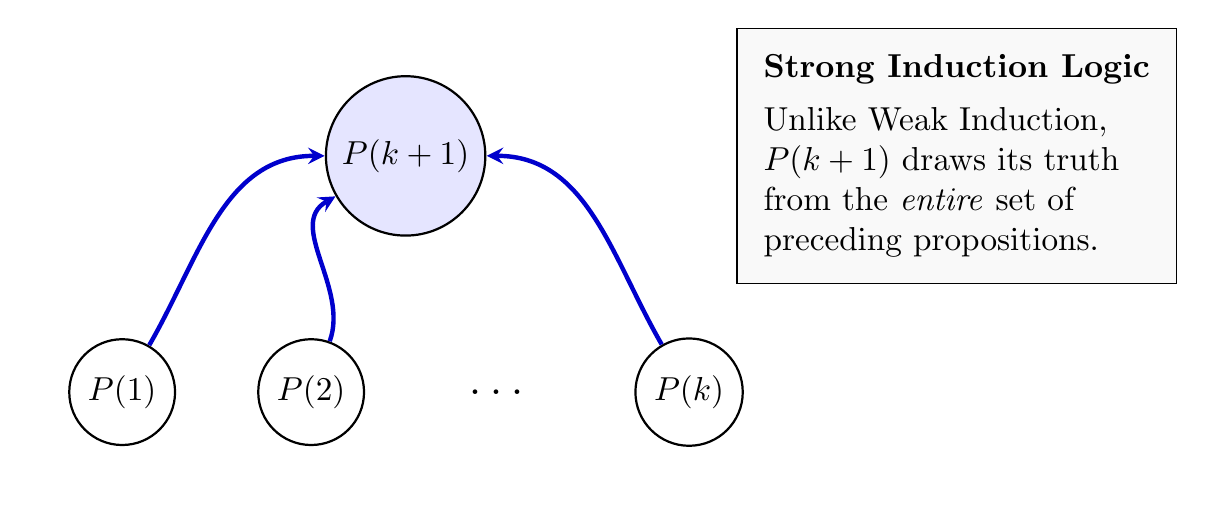
\begin{tikzpicture}[scale=1.2, transform shape, >=stealth]
    % Background to ensure clean rendering
    \fill[white] (-1,-1) rectangle (10, 3.5);
    
    % Nodes
    \node[draw, circle, thick, minimum size=1cm] (p1) at (0,0) {$P(1)$};
    \node[draw, circle, thick, minimum size=1cm] (p2) at (2,0) {$P(2)$};
    \node (dots) at (4,0) {\Large $\dots$};
    \node[draw, circle, thick, minimum size=1cm] (pk) at (6,0) {$P(k)$};
    
    \node[draw, circle, thick, fill=blue!10, minimum size=1.2cm] (pk1) at (3,2.5) {$P(k+1)$};
    
    % Arrows for Strong Induction
    \draw[->, ultra thick, blue!80!black] (p1) to[out=60, in=180] (pk1);
    \draw[->, ultra thick, blue!80!black] (p2) to[out=70, in=210] (pk1);
    \draw[->, ultra thick, blue!80!black] (pk) to[out=120, in=0] (pk1);
    
    % Single-Node Multiline Legend
    \node[align=left, anchor=west, draw, inner sep=8pt, fill=gray!5] at (6.5, 2.5) {
        \textbf{Strong Induction Logic}\\[4pt]
        Unlike Weak Induction,\\
        $P(k+1)$ draws its truth\\
        from the \textit{entire} set of\\
        preceding propositions.
    };
\end{tikzpicture}
\end{center}
\vspace{1em}

\subsection{Heuristics \& "Cheats"}
\begin{itemize}
    \item \textbf{The "Look-Back" Rule:} If a recurrence relation defines $a_n$ using $a_{n-1}$ and $a_{n-2}$, you \textit{must} use Strong Induction, and you \textit{must} have exactly 2 base cases.
    \item \textbf{The Frobenius Shortcut:} For any two relatively prime integers $a, b$, the largest integer that \textit{cannot} be expressed as $ax + by$ (for $x,y \ge 0$) is $ab - a - b$. All integers strictly greater than this bound can be formed.
\end{itemize}

\subsection{Pitfalls \& Fallacies}
\begin{itemize}
    \item \textbf{Insufficient Base Cases:} The most common fatal error in Strong Induction. If your inductive step requires looking back $c$ steps (e.g., $k-2$), you must manually prove $c$ consecutive base cases.
    \item \textbf{The "All Horses are the Same Color" Fallacy:} Assuming that the intersection of two sets is non-empty when transitioning from the base case to the inductive step. Always manually check $n=1 \to n=2$ or $n=2 \to n=3$ to ensure the logic doesn't break down at the boundary.
\end{itemize}

% ==========================================
% PART 5: CONCEPTUAL SYNTHESIS
% ==========================================
\section{Part 5: Conceptual Synthesis and The "Big Picture"}

\subsection{A) Thematic Connections}
The central theme of this chapter is \textbf{State-Space Dependency}. In standard calculus, a derivative at a point only depends on the infinitesimal neighborhood around that point (a Markovian property). Strong Induction introduces a framework where the current state of a system depends on its \textit{entire historical trajectory}. This bridges abstract logic to the concept of "memory" in stochastic processes and algorithms.

\subsection{B) Forward and Backward Links}
\begin{itemize}
    \item \textbf{Backward Link:} Strong induction is the logical extension of the Well-Ordering Principle from basic set theory. It translates a static property of sets (having a minimum) into a dynamic tool for proving infinite sequences.
    \item \textbf{Forward Link:} This concept is the absolute bedrock for \textbf{Dynamic Programming} in Computer Science and \textbf{Backward Induction} in Game Theory. Understanding how to build a truth from all previous sub-problems is exactly how algorithms like Bellman-Ford or Viterbi operate.
\end{itemize}

% ==========================================
% PART 6: ABSTRACT REAL-WORLD MODELING
% ==========================================
\section{Part 6: Abstract Real-World Modeling (AI, ML, \& Quant Finance)}

\subsection{A) Concrete Scenarios}
\begin{enumerate}
    \item \textbf{Reinforcement Learning (Bellman Equations):} In AI, an agent learns the optimal policy by evaluating the Value Function $V(s)$. Proving the convergence of Value Iteration relies on strong induction over the time horizon, as the value at step $k+1$ depends on the maximum expected values of all possible subsequent states computed in previous steps.
    \item \textbf{Quantitative Finance (Derivative Pricing):} In discrete-time stochastic calculus, pricing an American or European Option via a Binomial Tree requires Backward Induction. The price of the derivative at time $t=0$ is proved to be arbitrage-free by strongly inducting backward from the expiration date $t=T$.
\end{enumerate}

\subsection{B) Model Problem Setup: Binomial Option Pricing}
Let us formalize the Binomial Option Pricing Model using a probability space $(\Omega, \F, \Prob)$. We wish to price a European Call Option with strike $K$ expiring at time $T$.

\textbf{State Space \& Random Variables:}
Let the stock price at time $t$ be $S_t$. At each time step $\Delta t$, the stock can move up by a factor $u$ or down by a factor $d$. Thus, $S_{t+1} \in \{uS_t, dS_t\}$.
Let $r$ be the risk-free interest rate. We define the risk-neutral probability measure $\Q$ such that the discounted stock price is a martingale:
\[ \E^\Q [S_{t+1} \mid \F_t] = e^{r \Delta t} S_t \]
This yields the risk-neutral probability $q = \frac{e^{r \Delta t} - d}{u - d}$.

\textbf{The Induction Model:}
Let $V_t(s)$ be the price of the option at time $t$ given $S_t = s$. The terminal payoff at $t=T$ is known:
\[ V_T(s) = \max(s - K, 0) \]
We claim that for all $t \in \{T, T-1, \dots, 0\}$, the arbitrage-free price is given by:
\[ V_t(s) = e^{-r \Delta t} \E^\Q [V_{t+1}(S_{t+1}) \mid S_t = s] \]
\textit{Proof Sketch via Strong (Backward) Induction:}
The base case is $t=T$, which is trivially true by the contract definition. Assume the pricing formula holds for all times $i$ such that $t < i \le T$. To find $V_t(s)$, we construct a riskless portfolio $\Pi_t$ consisting of $\Delta$ shares of stock and $B$ in the risk-free bank account to replicate $V_{t+1}$. Because the values of $V_{t+1}(us)$ and $V_{t+1}(ds)$ are completely known and fixed by our strong inductive hypothesis, the system of linear equations for $\Delta$ and $B$ is perfectly determined. Discounting the riskless portfolio yields the expectation under $\Q$, proving the formula for $t$.

% ==========================================
% PART 7: COMMON VARIATIONS
% ==========================================
\section{Part 7: Common Variations and Untested Concepts}

A critical concept often taught alongside Strong Induction but missing from the provided homework is \textbf{Structural Induction}. While standard induction operates on $\N$, structural induction operates on recursively defined mathematical structures, such as graphs, trees, or logical formulas.

\textbf{Missing Concept: Structural Induction on Binary Trees}
\begin{theorem}
    For any full binary tree $T$ (where every internal node has exactly 2 children), the number of leaves $L(T)$ is exactly one more than the number of internal nodes $I(T)$. That is, $L(T) = I(T) + 1$.
\end{theorem}
\begin{proof}
    We proceed by structural induction on the tree $T$.
    
    \textbf{Base Case:} Let $T$ be a tree consisting of a single node (the root). This node is a leaf, so $L(T) = 1$. It has no children, so it is not an internal node, meaning $I(T) = 0$. Thus, $1 = 0 + 1$, and the base case holds.
    
    \textbf{Inductive Step:} Assume the theorem holds for any full binary trees $T_1$ and $T_2$. We construct a new full binary tree $T$ by taking a new root node and attaching $T_1$ as its left subtree and $T_2$ as its right subtree.
    The leaves of $T$ are simply the combined leaves of $T_1$ and $T_2$:
    \[ L(T) = L(T_1) + L(T_2) \]
    The internal nodes of $T$ are the internal nodes of $T_1$, the internal nodes of $T_2$, plus the new root node:
    \[ I(T) = I(T_1) + I(T_2) + 1 \]
    By our structural inductive hypothesis, $L(T_1) = I(T_1) + 1$ and $L(T_2) = I(T_2) + 1$. Substituting these into the leaf equation:
    \begin{align*}
        L(T) &= (I(T_1) + 1) + (I(T_2) + 1) \\
        &= (I(T_1) + I(T_2) + 1) + 1 \\
        &= I(T) + 1
    \end{align*}
    This completes the proof.
\end{proof}

% ==========================================
% PART 8: ADVANCED DIAGNOSTIC TESTING
% ==========================================
\section{Part 8: Advanced Diagnostic Testing: "Find the Flaw"}

Below are five proofs that appear rigorous but contain a subtle, fatal flaw. Your task as a student is to identify the error. The solutions are provided at the end.

\subsection{Flawed Proofs}

\textbf{Problem 1:} Prove that all horses are the same color.
\begin{proof}
    Let $P(n)$ be the statement that in any set of $n$ horses, all horses are the same color.
    Base case ($n=1$): In a set of 1 horse, all horses are trivially the same color.
    Inductive step: Assume $P(k)$ is true. Consider a set of $k+1$ horses. Remove the first horse; the remaining $k$ horses must be the same color by the hypothesis. Put the first horse back and remove the last horse; the remaining $k$ horses are the same color. Since the middle horses were in both sets, all $k+1$ horses must share this color. Thus $P(k+1)$ is true.
\end{proof}

\textbf{Problem 2:} Prove that $a^n = 1$ for all non-negative integers $n$.
\begin{proof}
    Base case ($n=0$): $a^0 = 1$, which is true.
    Strong Inductive step: Assume $a^i = 1$ for all $0 \le i \le k$. We prove for $k+1$:
    \[ a^{k+1} = \frac{a^k \cdot a^k}{a^{k-1}} \]
    By the strong inductive hypothesis, $a^k = 1$ and $a^{k-1} = 1$. Thus, $a^{k+1} = \frac{1 \cdot 1}{1} = 1$.
\end{proof}

\textbf{Problem 3:} Prove that every integer $n \ge 2$ is prime.
\begin{proof}
    Base case ($n=2$): 2 is prime.
    Strong Inductive step: Assume all integers $2 \le i \le k$ are prime. Consider $k+1$. If $k+1$ is prime, we are done. If $k+1$ is composite, it can be factored as $a \cdot b$. Since $a, b \le k$, by the inductive hypothesis, $a$ and $b$ are prime. Therefore, $k+1$ is made of primes, so it is prime.
\end{proof}

\textbf{Problem 4:} Prove that the Fibonacci sequence satisfies $F_n < 2^n$ for all $n \ge 1$.
\begin{proof}
    Base case ($n=1$): $F_1 = 1 < 2^1 = 2$.
    Strong Inductive step: Assume $F_i < 2^i$ for all $1 \le i \le k$.
    For $k+1$: $F_{k+1} = F_k + F_{k-1}$.
    By hypothesis, $F_k < 2^k$ and $F_{k-1} < 2^{k-1}$.
    Thus, $F_{k+1} < 2^k + 2^{k-1} < 2^k + 2^k = 2^{k+1}$.
\end{proof}

\textbf{Problem 5:} Prove that any amount of postage greater than 7 cents can be formed using 3-cent and 5-cent stamps.
\begin{proof}
    Base case ($n=8$): $8 = 3(1) + 5(1)$.
    Inductive step: Assume true for $8 \le i \le k$. For $k+1$, we look at $(k+1) - 3 = k-2$. By the strong inductive hypothesis, $k-2$ can be formed by 3 and 5-cent stamps. Add one 3-cent stamp to get $k+1$.
\end{proof}

\subsection{Solution Key: The Flaws Revealed}
\begin{enumerate}
    \item \textbf{Flaw in 1:} The intersection of the two sets of $k$ horses is empty when $k+1 = 2$. The logic "the middle horses were in both sets" fails because there are no middle horses when transitioning from $n=1$ to $n=2$.
    \item \textbf{Flaw in 2:} The formula $a^{k+1} = \frac{a^k \cdot a^k}{a^{k-1}}$ requires $k-1 \ge 0$. When $k=0$ (trying to prove $n=1$), the formula references $a^{-1}$, which is outside the domain of our base case $n=0$.
    \item \textbf{Flaw in 3:} A fundamental logical fallacy (Equivocation). The proof correctly deduces that $k+1$ is a product of primes, but then falsely concludes that being a product of primes makes the number itself prime.
    \item \textbf{Flaw in 4:} Missing base case. The recurrence $F_{k+1} = F_k + F_{k-1}$ looks back two steps, meaning the proof requires \textit{two} base cases ($n=1$ and $n=2$). The proof only provided $n=1$.
    \item \textbf{Flaw in 5:} Insufficient base cases. The inductive step subtracts 3, meaning it requires 3 consecutive base cases ($n=8, 9, 10$). Because $n=9$ and $n=10$ were not proven, the step $k+1=9 \implies k-2=6$ fails because 6 is outside the inductive hypothesis domain ($i \ge 8$).
\end{enumerate}

\end{document}